% ==================================================
% CHAPTER 4: Validating x-ray alignment parameters with cosmic muon data %
% ==================================================

\chapter{Validating x-ray alignment parameters with cosmic muon data}
\label{chap:comparison}
% Edit count: Lia - 0, Brigitte - 0

% --------------------------------------------------
\section{Presentation of theoretical method for comparison}
% --------------------------------------------------

The goal of this work is to validate the alignment parameters extracted from the x-ray data with cosmics data. The complication is that the x-ray dataset provides absolute local offsets while the cosmics dataset provides relative local offsets, which cannot be compare directly. The solution is to analyze the x-ray data in the same relative coordinate system as the cosmics data.

%TODO : decide on a consistent way to call the x-ray centroids
%TODO : determine if the description of equation 1.1 is suitably general enough to describe the x-ray data

The measured x-ray beam profile centers provided were systematically affected by local offsets in the same way as cosmics, as described by equation \ref{eqn:local_translation}. Therefore, if a 2-layer track is abstracted from the beam profile centers on each layer, and the residual calculated on a third layer, that residual should match the mean cosmics residual in that area. The track is "abstracted" because the beam profile center is actually the Gaussian mean of all selected cluster centroids that were recorded during the x-ray data taking period. This was the best analysis method because since the x-rays cause signal in the chamber via the photoeffect, there were not individual "x-ray tracks" to record. In fact the x-ray data was collected separately for each layer. However, since the effect of local offsets on the x-ray residuals was the same, the difference in algorithm between x-ray and cosmics analysis did not matter. 

Therefore, for each x-ray survey position, the x-ray residual was calculated for all possible tracking combinations (which required an x-ray beam profile on at least three layers). The position of the x-ray residuals are shown as black dots over figure~\ref{fig:res_mean_th2_L2_F13} and \ref{fig:res_mean_th2_L4_F13}. Note that the mean of cosmics residuals around the x-ray points were calculated in bins exactly centered on the nominal x-ray gun position, unlike in figure~\ref{fig:res_mean_th2}.

Correlation plots were used to visualize the correlation between the x-ray and cosmics residuals. An example for QL2.P.11 is shown in figure~\ref{fig:correlation}.

\begin{figure}
    \centering
    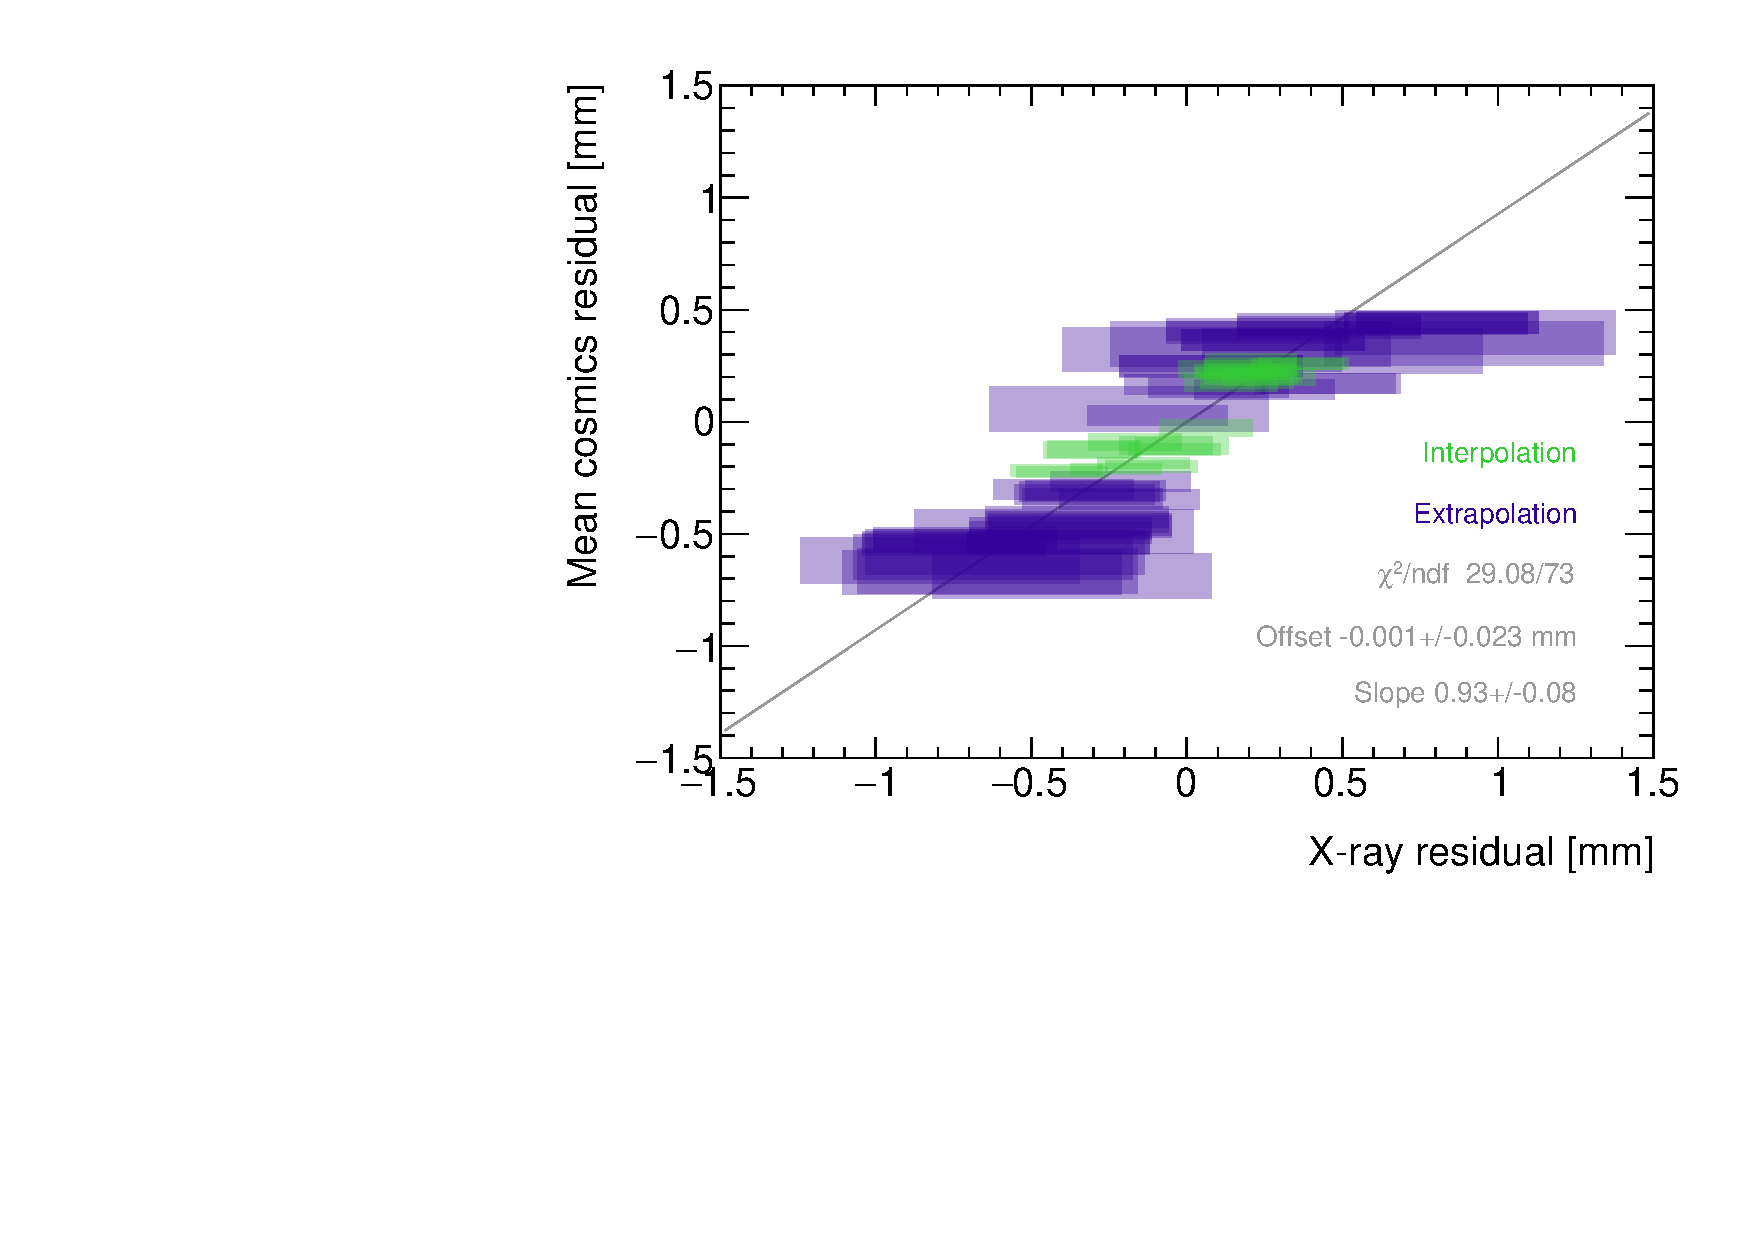
\includegraphics[width = \textwidth]{figures/figure_QL2P11_3100V_2021-08-05_QL2P11_local_cosmic_and_xray_data_correlation_plot.pdf}
    \caption{Correlation plot between x-ray and cosmics residuals for all tracking combinations for QL2.P.11.}
    \label{fig:correlation}
\end{figure}

First, the fitted slope and offset in figure~\ref{fig:correlation} show that the two datasets largely supported one another for QL2.P.11. However, the magnitude of the uncertainties in the x-ray residuals is large, since it comes from polating the measured x-ray beam centers, which have uncertainty of \SI{120}{\micro\meter} each. The large uncertainty sets a limit on the sensitivity of the analysis, for if the relative offsets of a quadruplet are smaller than the x-ray residual uncertainties, no conclusion about the correlation can be drawn, like for QL2.P.8 (figure~\ref{fig:no_correlation}).

\begin{figure}
    \centering
    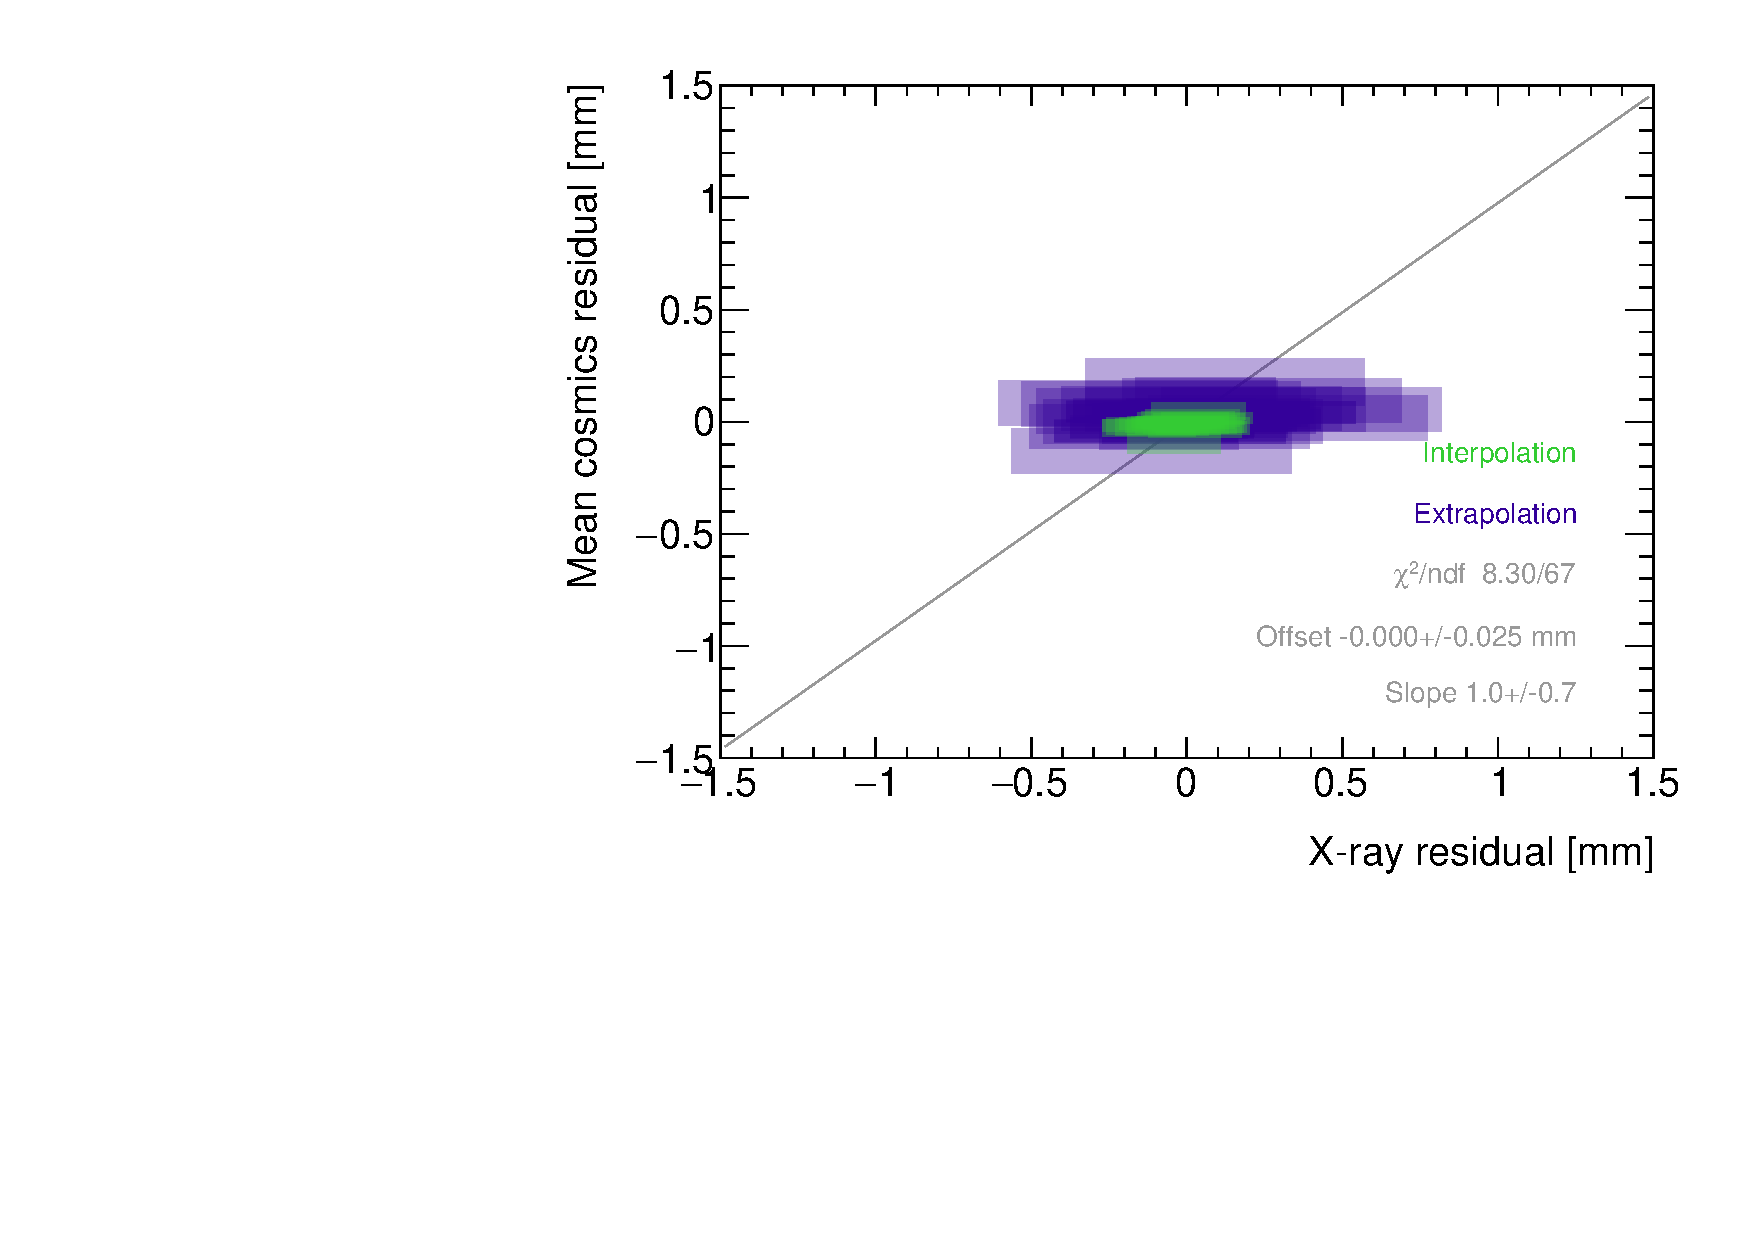
\includegraphics[width = \textwidth]{figures/figure_QL2P08_3100V_2021-08-16_QL2P08_local_cosmic_and_xray_data_correlation_plot.pdf}
    \caption{Correlation plot between x-ray and cosmics residuals for all tracking combinations for QL2.P.8.}
    \label{fig:no_correlation}
\end{figure}

Several quadruplets were tested for each geometries: QL2P, QL2C, and QS3P, and the conclusions above held. 

There are two patterns in the residuals on the scatter plot. First, residuals calculated through extrapolation tend to be larger because the extrapolation lever arm can produce more extreme values. Second, the pattern of points in figure~\ref{fig:correlation} is slightly mirrored. \textcolor{red}{This is exactly the correlation expected since each residual is the result of the same set of misalignment on each layers. Some tracking combinations naturally mirror each other, like extrapolating to layer 1 with layers 2 and 3 as reference, or extrapolating to layer 3 with 1 and 2 as reference.} \textit{Draw this out}.

% Comparing x-ray and cosmics residuals is precisely what was done with the new software package \package{strip_position_analysis}. Several quadruplets of each Canadian geometry were tested using this method, and every possible tracking combination was used to get enough comparison points to check the correlation. 

% --------------------------------------------------
\section{Limitations}
% --------------------------------------------------
An x-ray gun position was only useful if data was recorded on at least 3 layers since this is the minimum required to calculate a residual. 
- limited by position of alignment platforms
- smaller quads have smaller number of platforms
- edge wires, wire supports, and VMM boundaries affect data
Ideally, I would report the average number of gun positions with at least three layers per quadruplet, and the average number of residuals that go on the correlation plot.

